

Na verdade, o coeficiente de confiança de $J$ é dada por
\begin{equation}
\inf_{\theta \in \Theta} \left\{ \mathbb{P}_\theta \left[ \theta \in [T_L(x), T_U(x)] \right] \right\}
\end{equation}

Na maioria das aplicações, a probabilidade de cobertura não dependerá do parâmetro e será equivalente ao coeficiente de cobertura.

\textbf{Q (5.1)} Sejam 
\[
J_1 = (X_1 - 1,96; X_1 + 1,96)
\]
e 
\[
J_2 = \left( \bar{X} - \frac{1,96}{\sqrt{2}}, \bar{X} + \frac{1,96}{\sqrt{2}} \right)
\]
para $\mu$, dois intervalos aleatórios tais que $X_1, X_2 \sim N(\mu, 1)$ e 
\[
\bar{X} = \frac{X_1 + X_2}{2}.
\]
Encontre as probabilidades de cobertura de $J_1$ e $J_2$.

\textbf{Solução}

\begin{equation}
\mathbb{P}_\mu \{ \mu \in J_1 \} = \mathbb{P}_\mu \{ \mu \in (X_1 - 1,96; X_1 + 1,96) \}
\end{equation}

\begin{equation}
= \mathbb{P}_\mu \{ X_1 - 1,96 < \mu < X_1 + 1,96 \}
\end{equation}

\begin{equation}
= \mathbb{P}_\mu \{ (X_1 - \mu) \leq 1,96 \ \cap \ (X_1 - \mu) \geq -1,96 \}
\end{equation}

\begin{equation}
\mathbb{P}_\mu \{ \mu \in J_2 \} = \mathbb{P}_\mu \{ |X_1 - \mu| < 1,96 \}
\end{equation}

\begin{equation}
= \mathbb{P}_\mu \{ |Z| < 1,96 \}
\end{equation}

\begin{equation}
= \Phi(1,96) - \Phi(-1,96)
\end{equation}

\[
= 95\%
\]

\begin{center}
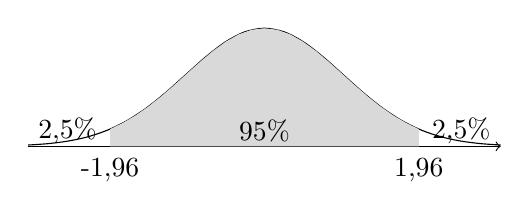
\begin{tikzpicture}
\draw[->] (-3,0) -- (3,0);
\draw[domain=-3:3,smooth,variable=\x] plot ({\x},{1.5*exp(-\x*\x/2)});
\draw[dashed] (-1.96,0) -- (-1.96,{1.5*exp(-1.96*1.96/2)});
\draw[dashed] (1.96,0) -- (1.96,{1.5*exp(-1.96*1.96/2)});
\fill[gray!30] (-1.96,0) -- plot[domain=-1.96:1.96] ({\x},{1.5*exp(-\x*\x/2)}) -- (1.96,0) -- cycle;
\node at (0,0.2) {95\%};
\node at (-2.5,0.2) {2,5\%};
\node at (2.5,0.2) {2,5\%};
\node at (-1.96,-0.3) {-1,96};
\node at (1.96,-0.3) {1,96};
\end{tikzpicture}
\end{center}

